\documentclass[10pt]{amsproc}
\usepackage{hyperref,color,ytableau,MnSymbol,graphicx}
\newtheorem{theorem}{Theorem}[subsection]
\newtheorem{lemma}[theorem]{Lemma}
\newtheorem{corollary}[theorem]{Corollary}
\theoremstyle{definition}
\newtheorem{definition}[theorem]{Definition}
\theoremstyle{remark}
\newtheorem{remark}[theorem]{Remark}
\newtheorem{example}[theorem]{Example}
\newcommand{\rowins}{\mathrm{RINS}}
\newcommand{\ins}{\mathrm{INSERT}}
\newcommand{\del}{\mathrm{DELETE}}
\newcommand{\Tab}{\mathrm{Tab}}
\newcommand{\rc}[1]{\mathbf{#1}}
\newcommand{\rd}{\mathrm{read}}
\newcommand{\wt}{\mathrm{wt}}
\newcommand{\shape}{\mathrm{shape}}
\newcommand{\pl}{\mathrm{pl}}
\newcommand{\ttab}{\mathrm{Tab}^\dagger}
\newcommand{\tr}{\mathrm{R}^\dagger}
\newcommand{\rp}{\mathbf{R}^+}
\newcommand{\rsk}{\mathrm{RSK}}
\newcommand{\ot}{\leftarrow}
\newcommand{\infl}{\mathrm{INFL}}
\newcommand{\supp}{\mathrm{supp}}
\title{A Timed Version of the Plactic Monoid}
\author{Amritanshu Prasad}
\address{The Institute of Mathematical Sciences, Chennai}
\address{Homi Bhabha National Institute, Mumbai}
\begin{document}
\maketitle
\begin{abstract}
  
\end{abstract}
\section{Introduction}
The plactic monoid was introduced by Lascoux and Sch\"utzenberger \cite{plaxique} to give a simple and elegant proof of the Littlewood-Richardson rule, based on an outline given by Robinson \cite{robinson-algo}, and ideas further deeloped by Schensted\cite{schensted} and Knuth \cite{knuth}, involving bijective correspondences involving words and semistandard tableaux.

It is now well-understood that these bijective correspondences are really restictions to lattice points of certain volume-preserving piecewise linear bijections between convex polyhedra \cite{kir-trop}.
The importance of this viewpoint is borne out in the work of Knutson and Tao, who proved the saturation of the monoid of triples $(\lambda, \mu, \nu)$ of integer partitions such that the trivial representation occurs in the tensor product $V_\lambda\otimes V_\mu\otimes V_\nu$ of representations of $GL_n(\mathbf C)$.
This led to the resolution of \emph{Horn's conjecture} on the possible sets of eigenvalues of a sum of Hermitian matrices (see \cite{knutsontaojams,knutsontaonotices}).

The goal of this article is to lay the algorithmic foundations for piecewise linear correspondences interpolating bijections involving tableaux.
This is done by generalizing the plactic monoid from the frameword of the free monoid of words to the setting of \emph{timed words}.
The latter were introduced by Alur and Dill \cite{alur-dill} in their approach to the formal verification of real-time systems using timed automata.
While words represent a sequence of events, timed words represent a sequence of events where the time of occurence of each event is also recorded.
We use a finite version of their definition of timed words.
While each letter occurs discretely (a certain number of times) in a classical word, it appears for a positive duration (which is a real number) in a timed word 

In Section~\ref{sec:timed-tableaux} we introduce the timed versions of semistandard Young tableaux (called \emph{timed tableaux}). 
Schensted's insertion algorithm is generalized to timed tableaux in Section~\ref{sec:timed-insertion}.
Greene invariants of timed words are introduces in Section~\ref{sec:timed-greene-invar}.
Timed versions of Knuth relations are introduced in Section~\ref{sec:timed-knuth-equiv}. 
These relations are conceptually very similar to the relations introduced by Knuth in \cite{knuth}. 
However, it was a delicate task to arrive at relations that are at once simple enough so that one can show that they preserve Greene invariants (Lemma~\ref{lemma:Knuth-Greene}) and at the same time powerful enough to transform any timed word to its insertion tableau (Lemma~\ref{lemma:reduction-to-tab}).
With this groundwork, the extension of Greene's theorem to timed words is routine (Theorem~\ref{theorem:timed-version-greene}).

Standard properties of Knuth equivalence, such as the existence of a unique tableau in each Knuth class, and the characterization of Knuth equivalence in terms of Greene invariants are extended to timed words in Sections~\ref{sec:tabl-knuth-equiv} and \ref{sec:char-timed-knuth}.

The RSK algorithm \cite{knuth} is extended from integer matries in Sections~\ref{sec:defin-using-timed} and \ref{sec:insert-record-algor}.
Viennot's light-and-shadows version of the Robinson-Schensted correspondence, which was extended to integer matrices in \cite{rtcv}, is now extended to real matrices.
The piecewise linear nature of these algorithms can be easily seen from the timed version of Greene's theorem.

All the algorithms described here are straightforward to implement 
\section{Insertion in Timed Tableaux}
\label{sec:insertion}
\subsection{Timed Tableaux}
\label{sec:timed-tableaux}
Let $A_n=\{1,\dotsc,n\}$, to be thought of as a linearly ordered alphabet.
\begin{definition}
  [Timed Word]
  \label{definition:timed-word}
  A timed word of length $r$ in the alphabet $A_n$ is a piecewise-constant right-continuous function $w:[0,r)\to A_n$.
  We write $l(w)=r$.
  In other words, for some finite sequence $0=r_0<r_1<\dotsc<r_k=r$ of transition points, and letters $c_1,\dotsc, c_k$ in $A$, $w(x) = c_i$ if $r_{i-1}\leq x < r_i$.
  Given such a function, we write
  \begin{equation}
    \label{eq:exp_not}
    w = c_1^{t_1} c_2^{t_2}\dotsb c_k^{t_k}, \text{ },
  \end{equation}
  where $t_i = r_i-r_{i-1}$.
  We call this the \emph{exponential string} for $w$.
  The weight of $w$ is the vector:
  \begin{displaymath}
    \wt(w) = (m_1,\dotsc,m_n),
  \end{displaymath}
  where $m_i$ is the Lebesgue measure of the pre-image of $i$ under $w$, i.e., $m_i=\mathrm{meas}(w^{-1}(i))$.
\end{definition}
The exponential string, as defined above, is not unique; if two successive letters $c_i$ and $c_{i+1}$ are equal, then we can merge them, replacing $c_i^{t_i}c_{i+1}^{t_{i+1}} = c_i^{t_i+t_{i+1}}$.

The above definition is a finite variant of Definition~3.1 of Alur and Dill~\cite{alur-dill}, where $r=\infty$, and there is an infinite increasing sequence of transition points.

Given timed words $w_1$ and $w_2$, their \emph{concatenation} is defined in the most obvious manner---their exponential strings are concatenated (and if necessary, successive equal values merged).
The monoid formed by all timed words in an alphabet $A_n$, with product defined by concatenation, will be denoted by $A_n^\dagger$.
The submonoid of $A_n^\dagger$ consisting of timed words where the exponents $t_1,t_2,\dotsc,t_k$ in exponential string (\ref{eq:exp_not}) are integers is the free monoid $A_n^*$ of words in the alphabet $A_n$ (see e.g., \cite[Chapter~1]{comb-words}).
\begin{definition}
  [Timed Subword]
  \label{definition:timed-subword}
  Given a timed word $w:[0,r)\to A_n$, and $S\subset [0,r)$ a finite disjoint union of intervals of the form $[a, b)\subset [0,r)$, the timed subword of $w$ with respect to $S$ is defined as the timed word:
  \begin{displaymath}
    w_S(t) = w(\inf\{u\in [0,r)\mid \mathrm{meas}([0,u)\cap S) \geq t\}) \text{ for } 0\leq t < \mathrm{meas}(S).
  \end{displaymath}
  Intuitively, $w_S$ is obtained from $w$ by cutting out the segments that are outside $S$.
  Given two words $v$ and $w$, $v$ is said to be a subword of $w$ if there exists $S\subset [0,r)$ as above such that $v=w_S$.
  Subwords $v_1,\dotsc,v_k$ of $w$ are said to be pairwise disjoint if there exist pairwise disjoint subsets $S_1,\dotsc,S_k$ as above such that $v_i=w_{S_i}$ for $i=1,\dotsc,k$.
\end{definition}
\begin{definition}[Timed Row]
A \emph{timed row} in the alphabet $A_n$ is a weakly increasing timed word in $A_n^\dagger$.
In exponential notation every timed row is of the form $1^{t_1}\dotsb n^{t_n}$ where $t_i\geq 0$ for $i=1,\dotsc,n$.
The set of all timed rows in $A_n^\dagger$ is denoted $\tr_n$.
The set of all timed rows of length $l$ is denoted $\tr_n(l)$.
\end{definition}
\begin{definition}[Row Decomposition]
Every timed word $w$ has a unique decomposition into rows:
\begin{displaymath}
  w = u_l u_{l-1}\dotsb u_1,
\end{displaymath}
such $u_i$ is a row for each $i=1,\dotsc,l$, and $u_iu_{i-1}$ is not a row for any $i=2,\dotsc,l$.
We shall refer to such a decomposition as the row decomposition of $w$.
\end{definition}
Given two rows $u$ and $v$, say that $u$ is dominated by $v$ (denoted $u\lhd v$) if
\begin{enumerate}
\item $l(u)\geq l(v)$, and
\item $u(t)<v(t)$ for all $0\leq t<l(v)$.
\end{enumerate}
\begin{definition}[Timed Tableau]\label{definition:timed-tableau}
  A timed tableau in $A_n$ is a timed word $w$ in $A_n$ with row decomposition $w=u_l u_{l-1}\dotsb u_1$ such that $u_1\lhd \dotsb \lhd u_l$.
  The shape of $w$ is the weakly decreasing tuple $(l(u_1),l(u_2),\dotsc,l(u_l))$ of positive real numbers (henceforth called a \emph{real partition}), and the weight of $w$ is the weight of $w$ as a timed word (see Definition~\ref{definition:timed-word}).
  The set of all timed tableau in $A_n$ is denoted $\ttab_n$.
  The set of all timed tableau of shape $\lambda$ is denoted $\ttab_n(\lambda)$.
  The set of all timed tableau of shape $\lambda$ and weight $\mu$ is denoted $\ttab_n(\lambda,\mu)$.
\end{definition}
The above is a direct generalization of the notion of the reading word of a tableau in the sense of \cite{Lascoux}.
\begin{example}
  \label{example:timed-tableau}
  $w=3^{0.8}4^{1.1}1^{1.4}2^{1.6}3^{0.7}$ is a timed tableau in $A_5$ of shape $(3.7,1.9)$ and weight $(1.4, 1.6, 1.5, 1.1,0)$.
\end{example}
\subsection{Timed Insertion}
\label{sec:timed-insertion}
Given a timed word $w$ and $0\leq a < b \leq l(w)$, according to Definition~\ref{definition:timed-subword}, $w_{[a, b)}$ is the timed word of length $b-a$ such that:
\begin{displaymath}
  w_{[a, b)}(t) = w(a+ t) \text{ for } 0\leq t<b-a.
\end{displaymath}
\begin{definition}[Timed row insertion]
  \label{definition:timed-row-insertion}
  Given a timed row $u$, the insertion $\rowins(u, c^{t_c})$ of $c^{t_c}$ into $u$ is defined as follows:
  if $w(t)\leq c$ for all $0\leq t < l(u)$, then
  \begin{displaymath}
    \rowins(w, c^{t_c}) = (\emptyset, wc^{t_c}).
  \end{displaymath}
  Otherwise, there exists $0\leq t < l(u)$ such that $w(t)>c$.
  Let
  \begin{displaymath}
    t_0 = \min\{0\leq t< l(u) \mid u(t)> c\}.
  \end{displaymath}
  Define
  \begin{displaymath}
    \rowins(u, c^{t_c}) =
    \begin{cases}
      (u_{[t_0, t_0+t_c)}, u_{[0, t_0)}c^{t_c} u_{[t_0+t_c, l(w))}) & \text{if } l(u) - t_0 > t_c,\\
      (u_{[t_0, l(u))}, u_{[0, t_0)} c^{t_c}) & \text{if } l(u) - t_0 \leq t_c.
    \end{cases}
  \end{displaymath}
  When $t=1$ and $u$ lies in the image of $A^*$ in $A^\dagger$, this coincides with the first step of the algorithm INSERT from Knuth \cite{knuth} where $c$ is inserted into a row:
  if $\rowins(u,c^1)=(v',u')$, then $u'$ is the new row obtained after insertion, $v'$ is the letter bumped out by $c$.

  If $v$ is a row of the form $c_1^{t_1}\dotsb c_k^{t_k}$.
  Define $\rowins(u,v)$ by induction on $k$ as follows:
  Having defined $(v',u')=\rowins(u,c_1^{t_1}\dotsb c_{k-1}^{t_{k-1}})$,
  let $(v'', u'')=\rowins(u',c_l^{t_k})$.
  Then define
  \begin{displaymath}
    \rowins(w,u) = (v'v'', u'').
  \end{displaymath}
\end{definition}
\begin{example}
  \label{example:timed-row-ins}
  $\rowins(1^{1.4}2^{1.6}3^{0.7},1^{0.7}2^{0.2})=(2^{0.7}3^{0.2},1^{2.1}2^{1.1}3^{0.5})$.
\end{example}
\begin{definition}
  [Timed Tableau Insertion]
  Let $w$ be a timed tableau with row decomposition $u_l\dotsc u_1$, and let $v$ be a timed row.
  Then $\ins(w, v)$, the insertion of $v$ into $w$ is defined as follows:
  first $v$ is inserted into $u_1$.
  If $\rowins(u_1,v)=(v_1',u_1')$, then $v_1'$ is inserted into $u_2$; if $\rowins(u_2,v_1')=(v_2',u_2')$, then $v_2'$ is inserted in $u_3$, and so on.
  This process continues, generating $v_1',\dotsc,v_l'$ and $u_1',\dotsc,u_l'$.
  $\ins(t,v)$ is defined to be $v_l'u_l'\dotsb u_1'$.
  It is quite possible that $v_l'=\emptyset$.
\end{definition}
\begin{example}
  If $w$ is the timed tableau from Example~\ref{example:timed-tableau}, then
  \begin{displaymath}
    \ins(w,1^{0.7}2^{0.2})=3^{0.7}4^{0.2}2^{0.7}3^{0.3}4^{0.9}1^{2.1}2^{1.1}3^{0.5}.
  \end{displaymath}
\end{example}
When the timed tableau $w$ lies in the image of $A_n^*$, then $\ins(w,c^1)$ is the same as the result of applying the algorithm $\text{INSERT}(c)$ from Knuth \cite{knuth} to the semistandard Young tableau $w$.
\begin{definition}
  Given real partitions $\lambda=(\lambda_1,\dotsc,\lambda_l)$ and $\mu=(\mu_1,\dotsc,\mu_{l-1})$, we say that $\mu$ \emph{interleaves} $\lambda$ if the inequalities
  \begin{displaymath}
    \lambda_1 \geq \mu_1 \geq \lambda_2 \geq \mu_2 \geq \dotsb \geq \lambda_{l-1}\geq \mu_{l-1}\geq \mu_l. 
  \end{displaymath}
  In other words, the successive parts of $\mu$ lie in-between the successive parts of $\lambda$.
\end{definition}
\begin{theorem}
  \label{theorem:tableauness-of-insertion}
  For any timed tableau $w$ in $A_n$ and any timed row $v$ in $A_n$, $\ins(w,v)$ is again a timed tableau in $A_n$.
  We have
  \begin{displaymath}
    \wt(\ins(w,v)) = \wt(w) + \wt(v),
  \end{displaymath}
  and $\shape(w)$ interleaves $\shape(\ins(w,v))$.
\end{theorem}
\begin{proof}
  We first prove that $\ins(w,v)$ is a timed tableau.
  For this purpose, by inserting in stages, one may assume that $v=c^t$ for some $c\in A_n$ and some $t>0$.
  Let $w$ have row decomposition $u_lu_{l-1}\dotsb u_1$.
  If $u_1(t)\leq c$ for all $0\leq t<l(u_1)$, then $u_1'=u_1c^t$, and $u_2'=u_2$, and so $u_1'\lhd u_2'$.
  Otherwise, when $c^t$ is inserted into $u_1$, $v_1'$ is a segment of $u_1$ corresponding to an interval $[t_0,t_0+\delta)$ such that $u_1(t_0)>c$.
  This segment in $u_1$ is replaced by a segment $c^\delta$ to obtain $u_1'$.
  Let $v_1'=c_1^{t_1}\dotsb c_k^{t_k}$ (so $c<c_1< \dotsb <c_k$) be the exponential notation for $v_1'$.

  Proceed by induction on $k$.
  If $k=1$, $v_1'=c_1^{t_1}$.
  Now $u_2(t_0)>u_1(t_0)=c_1$, so $c_1^{t_1}$ will displace a segment of $u_2$ that begins to the left of $t_0$ with $c_1^{t_1}$, and so $u_1'\lhd u_2'$.

  For $k>1$, perform the insertion of $c^t$ into $w$ in two steps, first inserting $c^{t_1}$, and then inserting $c^{t-t_1}$.
  If $(v_1'',u_1'')=\rowins(u_1,c^{t_1})$, then $v_1''=c_1^{t_1}$.
  Let $(v_2'',u_2'')=\rowins(u_2,v_1'')$.
  By the $k=1$ case, $u_1''\lhd u_2''$.
  
  Now $(c_2^{t_2}\dotsb c_k^{t_k},u_1')=\rowins(u_1'',c^{t-t_1})$, and $u_2'$ is obtained by inserting $c_2^{t_2}\dotsb c_k^{t_k}$ into $u_2''$.
  Therefore, by induction hypothesis, $u_1'\lhd u_2'$.
  Repeating this argument with the remaining rows shows that $u_1'\lhd u_2' \lhd \dotsb \lhd u_l'$, as required.

  To see that $\shape(w)$ interleaves $\shape(\ins(w,v))$, observe that $v_1'$ is a concatenation of segments of $u_1$.
  Write $v_1'=xy$, where $x$ consists of segments that come from $u_{1[0,l(u_2))}$ and $y$ consists of segments that come from $u_{1[l(u_2),l(u_1))}$.
  Then, from the arguments of the first part of this proof, the segments in $x$ will all replace segments of $u_2$, so if $(\tilde v,\tilde u_2)=\rowins(u_2,x)$, then $l(\tilde u_2)=l(u_2)$.
  Since $y$ is inserted into $\tilde u_2$ to obtain $u_2'$,
  Now $(v_2',u_2')=\rowins(\tilde u_2,y)$, whence 
  \begin{align*}
    l(u_2') &\leq l(\tilde u_2)+l(y)\\
    &\leq l(u_2)+[l(u_1)-l(u_2)]\\
    & = l(u_1).
  \end{align*}
  The same argument shows that $l(u_i')\leq l(u_{i-1})$ for $i>2$ as well, so that $\shape(w)$ interleaves $\shape(\ins(w,v))$.

  The assertion about weights is obvious.
\end{proof}
\begin{definition}
  [Insertion Tableau of a Timed Word]
  Let $w$ be a timed word with row decomposition $u_1\dotsb u_l$.
  The insertion tableau of $w$ is defined as:
  \begin{displaymath}
    P(w) = \ins(\dotsb\ins(\ins(u_1, u_2),u_3),\dotsc,u_l).
  \end{displaymath}
\end{definition}
\begin{example}
  If $w=3^{0.8}1^{0.5}4^{1.1}1^{0.9}2^{1.6}3^{0.7}1^{0.7}2^{0.2}$ has four rows in its row decomposition.
  $P(w)$ is calculated via the following steps:
  \begin{displaymath}
    \renewcommand{\arraystretch}{1.2}
    \begin{array}{|l|l|}
      \hline
      w & P(w)\\
      \hline
      3^{0.8} & 3^{0.8}\\
%      3^{0.8}1^{0.5} & 3^{0.5}1^{0.5}3^{0.3}\\
      3^{0.8}1^{0.5}4^{1.1} & 3^{0.5}1^{0.5}3^{0.3}4^{1.1}\\
%      3^{0.8}1^{0.5}4^{1.1}1^{0.9} & 3^{0.8}4^{0.6}1^{1.4}4^{0.5}\\
%      3^{0.8}1^{0.5}4^{1.1}1^{0.9}2^{1.6} & 3^{0.8}4^{1.1}1^{1.4}2^{1.6}\\
      3^{0.8}1^{0.5}4^{1.1}1^{0.9}2^{1.6}3^{0.7} & 3^{0.8}4^{1.1}1^{1.4}2^{1.6}3^{0.7}\\
%      3^{0.8}1^{0.5}4^{1.1}1^{0.9}2^{1.6}3^{0.7}1^{0.7} & 3^{0.7}2^{0.7}3^{0.1}4^{1.1}1^{2.1}2^{0.9}3^{0.7}\\
      3^{0.8}1^{0.5}4^{1.1}1^{0.9}2^{1.6}3^{0.7}1^{0.7}2^{0.2} & 3^{0.7}4^{0.2}2^{0.7}3^{0.3}4^{0.9}1^{2.1}2^{1.1}3^{0.5}\\
      \hline
    \end{array}
    \renewcommand{\arraystretch}{1}
  \end{displaymath}
\end{example}
\begin{definition}
  [Sch\"utzenberger Involution on Timed Words]
  \label{definition:schuetzenberger-involution}
  Given $w=c_1^{t_1}\dotsb c_k^{t_k}\in A_n^\dagger$, define
  \begin{equation}
    \label{eq:sharp}
    w^\sharp = (n-c_k+1)^{t_k} \dotsb (n-c_1+1)^{t_1},
  \end{equation}
  in effect, reversing both the order on the alphabet, and the positional order of letters in the timed word.
\end{definition}
\begin{lemma}
  \label{lemma:reverse-row-insertion}
  Let $u$ and $v$ be timed rows.
  Suppose $\rowins(u,v)=(v',u')$, and $l(v')=l(v)$.
  Then $\rowins({u'}^\sharp,{v'}^\sharp)=(v^\sharp,u^\sharp)$.
\end{lemma}
\begin{proof}
  It suffices to consider the case where $v=c^t$.
  The hypothesis $l(v')=l(v)$ implies that $t_0=\inf\{t\mid u(t)>c\}$ satisfies $0\leq t_0<l(u)-c$, and
  \begin{displaymath}
    u'=u_{[0,t_0)}c^tu_{[t_0+t,l(u))}, \text{ and } v'=u_{[t_0,t_0+t)}.
  \end{displaymath}
  Using induction as in the proof of Theorem~\ref{theorem:tableauness-of-insertion}, we may assume that $v'$ is constant, so $v'=d^t$ for some $d>c$.

  Now
  \begin{displaymath}
    {u'}^\sharp=u_{[t_0+t,l(u))}^\sharp (n-c+1)^t u_{[0,t_0)}^\sharp \text{ and } {v'}^\sharp=(n-d+1)^t.
  \end{displaymath}
  Since all the values of $u_{[t_0+t,l(u))}$ are greater than or equal to the last value of $d$, all the values of $u_{[t_0+t,l(u))}^\sharp$ are less than or equal to $n-d+1$.
  Moreover, $n-c+1>n-d+1$.
  It follows immediately from Definition~\ref{definition:timed-row-insertion} that $\rowins({u'}^\sharp,{v'}^\sharp)=(v^\sharp,u^\sharp)$.
\end{proof}
\begin{corollary}
  \label{corollary:row-insertion-bijection}
  The timed row insertion algorithm gives rise to a bijection:
  \begin{multline*}
    \rowins: \tr_n(r)\times \tr_n(s) \tilde\to \\\{(v',u')\in \tr_n(r+s-r')\times \tr_n(r')\mid r'\geq \max(r,s),\; u'\lhd v'\}. 
  \end{multline*}
\end{corollary}
\begin{proof}
  Suppose $(u,v)\in \tr_n(r)\times \tr_n(s)$, and $(v',u')=\rowins(u,v)$.
  Then $(u,v)$ can be recovered from $(v',u')$ (given the prior knowledge of $r$ and $s$) as follows:
  let $(v_1^\sharp, u_1^\sharp)=\rowins({u'_{[0,r)}}^\sharp, {v'}^\sharp)$.
  Then using Lemma~\ref{lemma:reverse-row-insertion}, $u$ and $v$ can be recovered as $u=u_1$, and $v=v_1u'_{[r,r')}$.
\end{proof}
\begin{theorem}[Timed Pieri Rule]
  \label{theorem:pieri}
  The timed insertion algorithm gives rise to a bijection:
  \begin{displaymath}
    \ins: \ttab_n(\lambda)\times \tr_n(r) \tilde\to \coprod_{\begin{smallmatrix}\text{$\lambda$ interleaves $\mu$}\\{l(\lambda)+r = l(\mu)}\end{smallmatrix}} \ttab_n(\mu)
  \end{displaymath}
\end{theorem}
\begin{proof}
  Let $\lambda=(\lambda_1,\dotsc,\lambda_l)$.
  Let $w\in \ttab_n(\lambda)$ have row decomposition $u_l\dotsb u_1$, and $x\in \tr_n(r)$.
  Suppose that $w'=\ins(w,x)$ has row decomposition $u'_{l+1}\dotsb u_1$ (with the possibility that $u_{l+1}=\emptyset$).
  We already know that $\shape(w)$ interleaves $\shape(w)$ (Theorem~\ref{theorem:tableauness-of-insertion}).
  Given timed rows $u'$ and $v'$ such that $u'\lhd v'$, and non-negative real numbers $r$ and $s$ such that $r\leq l(u')$, let $\rowins^{-1}_r(v',u')$ denote the unique pair of rows $(u,v)$ such that $l(u)=r$, $l(v)=s$, and $(v',u')=\rowins(u,v)$ (see Corollary~\ref{corollary:row-insertion-bijection}).
  Then the rows of $w$ can be recovered from $w'$ as follows:
  \begin{align*}
    (x_l, u_l) & = \rowins^{-1}_{\lambda_l}(u'_{l+1},u'_l),\\
    (x_{l-1},u_{l-1}) & = \rowins^{-1}_{\lambda_{l-1}}(x_l,u'_{l-1}),\\
    (x_{l-2},u_{l-2}) & = \rowins^{-1}_{\lambda_{l-2}}(x_{l-1},u'_{l-2}),\\
    &\vdots\\
    (x_1,u_1) & = \rowins^{-1}_{\lambda_1}(x_2,u'_1),
  \end{align*}
  and finally $x$ can be recovered as $x=x_1$.
\end{proof}
\begin{definition}
  [Deletion]
  \label{definition:deletion}
  Let $w'\in \ttab_n(\mu)$ and let $\lambda$ be a real partition that interleaves $\mu$.
  Then we write
  \begin{displaymath}
    \del_\lambda(w')=(v,w) \text{ if and only if } w\in \ttab_\lambda(n) \text{ and }\ins(w,v)=w'.
  \end{displaymath}
  The pair $(v,w)$ is computed from $w'$ and $\lambda$ by the algorithm described in the proof of Theorem~\ref{theorem:pieri}.
\end{definition}
\section{Greene's Theorem}
\label{sec:greene}
\subsection{Greene's Invariants for Timed Words}
\label{sec:timed-greene-invar}
\begin{definition}[Greene's Invariants for Timed Words]
  \label{definition:timed-Greene-invars}
  Given $w\in A_n^\dagger$, its $k$th Greene's invariant $a_k(w)$ is defined as the maximum possible sum of lengths of a set of $k$ pairwise disjoint subwords of $w$ (see Definition~\ref{definition:timed-subword}) that are all timed rows:
  \begin{multline*}
    a_k(w) = \max\{l(u_1)+\dotsb+l(u_k)\mid u_1,\dotsc,u_k \text{ are pairwise disjoint subwords,}\\ \text{and each $u_i$ is a timed row }\}
  \end{multline*}
\end{definition}
\begin{lemma}
  \label{lemma:tableau-shape-greene}
  If $w$ is a timed tableau of shape $\lambda=(\lambda_1,\dotsc,\lambda_l)$, then for each $1\leq k\leq l$,
  \begin{displaymath}
    a_k(w) = \lambda_1+\dotsb + \lambda_k.
  \end{displaymath}
\end{lemma}
\begin{proof}
  This proof is very similar to the proof of the corresponding result for ordinary tableaux \cite{Greene-schen,Lascoux}.
  Indeed, $u_1,\dotsc,u_k$ are pairwise disjoint subwords that are rows, so
  \begin{displaymath}
    a_k(w) \geq \lambda_1+\dotsb + \lambda_l.
  \end{displaymath}
  Conversely, any row subword of $w$ cannot have overlapping segments from two different rows $u_i$ and $u_j$ of $w$, because if $i>j$, then $u_i(t)>u_j(t)$, but in the row decomposition of $w$, $u_i$ occurs before $u_j$.
  Therefore, $k$ disjoint subwords can have length at most the sum of lengths of the largest $k$ rows of $w$, which is $\lambda_1+\dotsc+\lambda_k$.
\end{proof}
\subsection{Timed Knuth Equivalence and the Timed Plactic Monoid}
\begin{definition}
  [Timed Knuth Relations]
  \label{sec:timed-knuth-equiv}
  Assume that $x$, $y$ and $z$ are timed rows such that $xyz$ is also a timed row.
  The timed Knuth relations are given by:
  \begin{align}
    \tag{$\kappa_1$}
    \label{eq:tk1}
    xzy & \equiv zxy \text{ if } l(z)=l(y) \text{ and } \lim_{t\to l(y)^-} y(t)<z(0),\\
    \tag{$\kappa_2$}
    \label{eq:tk2}
    yxz & \equiv yzx\text{ if } l(x)=l(y) \text{ and } \lim_{t\to l(x)^-} x(t)<y(0).
  \end{align}
\end{definition}
\begin{definition}
  [Timed Plactic Monoid]
  \label{definition:timed-plactic-monoid}
  The timed plactic monoid $\pl(A_n)$ is the quotient $A^\dagger/\equiv$, where $\equiv$ is the congruence generated by the timed Knuth relations (\ref{eq:tk1}) and (\ref{eq:tk2}).
\end{definition}
In other words, two elements of $A^\dagger$ are said to differ by a Knuth move if they are of the form $uv_1w$ and $uv_2w$, where $v_1$ and $v_2$ are terms on opposite sides of one of the timed Knuth relations (\ref{eq:tk1}) and (\ref{eq:tk2}).
Knuth equivalence $\equiv$ is the equivalence relation generated by Knuth moves.
Since this equivalence is stable under left and right multiplication in $A^\dagger$, the concatenation product on $A^\dagger$ descends to a product on the set $\pl(A)$ of Knuth equivalence classes, giving it the structure of a monoid.
\begin{lemma}
  \label{lemma:sharp-moves}
  Then $v$ and $w$ differ by a Knuth move (\ref{eq:tk1}) if and only if $v^\sharp$ and $w^\sharp$ (see Definition~\ref{definition:schuetzenberger-involution}) differ by a Knuth move (\ref{eq:tk2}).
\end{lemma}
\begin{proof}
  When the involution $w\mapsto w^\sharp$ is applied to the Knuth relation (\ref{eq:tk1}), the Knuth relation (\ref{eq:tk2}) is obtained.
\end{proof}
\begin{lemma}
  \label{lemma:reduction-to-tab}
  Every timed word is Knuth equivalent to its timed insertion tableau.
\end{lemma}
\begin{proof}
  It suffices to show that, for every timed row $u$, and every term $c^t$, if $(v,u')=\rowins(u,c^t)$, then $uc^t\equiv vu'$.
  If $u(t)\leq c$ for all $0\leq t<l(u)$, there is nothing to show.
  Otherwise, a segment $v$ of $u$, beginning at $t_0$, and of length $t_1=\min(l(u)-t_0,t)$ is displaced by the segment $c^{t_1}$ of $c^t$.
  Write $u=u'vu''$.
  It suffices to show $u'vu''c^{t_1}\equiv vu'c^{t_1}u''$.
  But this can be done in two Knuth moves as follows (the segment to which the Knuth move is applied is underlined):
  \begin{displaymath}
    u'\underline{v u'' c^t} \equiv_{\kappa_2} u'\underline{vc^tu''} = \underline{u'vc^t}u'' \equiv_{\kappa_1} \underline{vu'c^t}u'',
  \end{displaymath}
  completing the proof of the lemma.
\end{proof}
\subsection{Knuth Equivalence and Greene's Invariants}
\label{sec:knuth-equiv-green}
\begin{lemma}
  \label{lemma:Knuth-Greene}
  If two timed words are Knuth equivalent, then they have the same Greene invariants.
\end{lemma}
\begin{proof}
  It suffices to prove that if two words differ by a Knuth move they have the same Greene invariants.
  For the Knuth move (\ref{eq:tk1}), suppose that $xyz$ is a timed row with $l(z)=l(y)$, and the last letter of $y$ is strictly less than the first letter of $z$.
  For any timed words $w$ and $u$, we wish to show that Greene's invariants coincide for $wxzyu$ and $wzxyu$.
  Now suppose that $v_1,\dotsc,v_k$ are pairwise disjoint row subwords of $wxzyu$ whose lengths add up to $a_k(wxzyu)$.
  We may write $v_i=w_ix_iz_iy_iu_i$ for each $i$, where $w_i,x_i,z_i,y_i$ and $u_i$ are row subwords of $w,x,z,y$ and $u$ respectively.

  Since the last letter of $y$ is strictly smaller than the first letter of $z$, it cannot be that $y_i\neq \emptyset$ and $z_i\neq \emptyset$ simultaneously for the same $i$.
  Renumber $v_1,\dotsc,v_k$ in such a way that $v_i=w_ix_iz_iu_i$ for $i=1,\dotsc,r$ and $v_i=w_ix_iy_iu_i$ for $i=r+1,\dotsc,k$.
  If $x_i=\emptyset$ for $i=1,\dotsc,r$, then all the $v_i$'s remain row subwords of $wzxyu$, and so $a_k(wzxyu)\geq a_k(wxzyu)$.
  If $y_i=\emptyset$ for $i=r+1,\dotsc,k$, then set
  \begin{align*}
    v_1'&=w_1x_1yu_1,\\
    v_i'&=w_ix_iu_i \text{ for } i=2,\dotsc,k.
  \end{align*}
  Then $v'_i$ are pairwise disjoint row subwords of $wzxyu$, and $l(v'_1)+\dotsb + l(v'_k)\geq l(v_1)+\dotsb l(v_k)$, since $l(y)=l(z)\geq l(z_1)+\dotsb + l(z_r)$.
  It follows that $a_k(wzxyu)\geq a_k(wxzyu)$.

  If at least one $x_i\neq \emptyset$ and one $y_i\neq\emptyset$, assume that $x_1$ has the least first letter among $x_1,\dotsc,x_r$, and that $y_k$ has the largest last letter among $y_{r+1},\dotsc,y_k$.
  Let $x_0$ be the row subword of $x$ obtained by concatenating the segments of $x_1,\dotsc,x_r$ in the order in which they appear in $x$ (so $x_0$ is a row of length $l(x_1)+\dotsb + l(x_r)$).
  Let $y_0$ be the row subword of $y$ obtained by concatenating the segments of $y_{r+1},\dotsc, y_k$ in the order in which they appear in $y$ (so $y_0$ is a row of length $l(y_{r+1})+\dotsb + l(y_k)$).
  Define
  \begin{align*}
    v'_1 &= w_1x_0y_0u_k\\
    v'_i &= w_iz_iu_i \text{ for }i=2,\dotsc,r,\\
    v'_i &= w_ix_iu_i \text{ for } i=r+1,\dotsc,k,\\
    v'_k &= w_kz_1u_1.
  \end{align*}
  Then $v'_1,\dotsc,v'_k$ are pairwise disjoint row subwords of $wzxyu$ with total length $l(v_1)+\dotsb+l(v_k)$, so $a_k(wzxyu)\geq a_k(wxzyu)$.
  The reverse inequality $a_k(wzxyu)\geq a_k(wxzyu)$ is obvious, since every row subword of $wzxyu$ is also a row subword of $wxzyu$.
  It follows that $a_k(wzxyu)=a_l(wxzyu)$ for all $k$.

  For the Knuth move (\ref{eq:tk2}) a similar argument can be given, however, a more elegant method is to use Lemma~\ref{lemma:sharp-moves}, noting that $a_k(w)=a_k(w^\sharp)$ for all $k\geq 1$ and all $w\in A_n^\dagger$.
\end{proof}
\subsection{The timed version of Greene' theorem}
\label{sec:timed-version-greene}
\begin{theorem}
  [Timed version of Greene's theorem]
  \label{theorem:timed-version-greene}
  For every $w\in A_n^\dagger$, if the timed tableau $P(w)$ has shape $\lambda=(\lambda_1,\dotsc,\lambda_l)$, then
  \begin{displaymath}
    a_k(w) = \lambda_1+\dotsb+\lambda_k \text{ for $k=1,\dotsc,l$}.
  \end{displaymath}
\end{theorem}
\begin{proof}
  Greene's theorem holds when $w$ is a timed tableau (Lemma~\ref{lemma:tableau-shape-greene}.
  By Lemma~\ref{lemma:Knuth-Greene}, Greene invariants remain unchanged under the timed versions of Knuth relations.
  By Lemma~\ref{lemma:reduction-to-tab}, every timed word is Knuth equivalent to its timed insertion tableau.
  Therefore, the Greene invariants of a timed word are given by the shape of its insertion tableau as stated in the theorem.
\end{proof}
\section{Knuth Equivalence Classes}
\label{sec:knuth-classes}
\subsection{Tableaux in Knuth Equivalence Classes}
\label{sec:tabl-knuth-equiv}
Given $w\in A_n^\dagger$, let $\bar w$ denote the word in $A_{n-1}^\dagger$ whose exponential string is obtained by removing all terms of the form $n^t$ with $t>0$ from the exponential string of $w$.
The word $\bar w$ is called the restriction of $w$ to $A_{n-1}$.
\begin{lemma}
  \label{lemma:restriction-interleaf}
  For every timed tableau $w\in A_n^\dagger$, $\bar w$ is also a timed tableau. Moreover, $\shape(\bar w)$ interleaves $\shape(w)$.
\end{lemma}
\begin{proof}
  Suppose $w$ has row decomposition $u_lu_{l-1}\dotsb u_1$.
  Since $n$ is the largest element of $A_n$, we may write $u_i=u'_in^{t_i}$ for some $t_i\geq 0$.
  Clearly $l(u_i)\geq l(u'_i)$.
  Since $w$ is semistandard, $l(u'_i)\geq l(u_{i+1})$ for $i=1,\dotsc,l-1$. 
  It follows that the shape of $w'$, which is $(l(u'_1),\dotsc,l(u'_l))$ interleaves the shape of $w$, which is $(l(u_1),\dotsc,l(u_l))$.
  Since $u_i\lhd u_{i+1}$, it follows that $u'_i\lhd u_{i+1}$ for $i=1,\dotsc,l-1$.
\end{proof}
\begin{lemma}
  \label{lemma:equivalence-restriction}
  If $v,w\in A_n^\dagger$ are Knuth equivalent, then their restrictions to $A_{n-1}$, $\bar v$ and $\bar w$ are Knuth equivalent in $A_{n-1}^\dagger$.
\end{lemma}
\begin{proof}
  Applying the restriction to $A_{n-1}$ map $w\mapsto \bar w$ to both sides of the Knuth relation (\ref{eq:tk1}) gives:
  $x\bar z y$ and $\bar z x y$.
  Write $y=y'y''$, where $l(y')=l(\bar z)$, we have
  \begin{displaymath}
    x\bar zy'y'' \equiv \bar zxy'y'',
  \end{displaymath}
  a Knuth relation in in $A_{n-1}^\dagger$.
  A similar argument works for the Knuth relation (\ref{eq:tk2}).
\end{proof}
\begin{theorem}
  \label{theorem:unique-timed-tableaux}
  Every Knuth equivalence class in $A_n^\dagger$ contains a unique timed tableau.
\end{theorem}
\begin{proof}
  The existence of a timed tableau in each Knuth equivalence class is ensured by Lemma~\ref{lemma:reduction-to-tab}.
  The proof of uniqueness is by induction on $n$.
  The base case, where $n=1$ is trivially true.
  Now suppose $v$ and $w$ are Knuth equivalent timed tableaux in $A_n^\dagger$.
  By Lemmas~\ref{lemma:restriction-interleaf} and~\ref{lemma:equivalence-restriction} $\bar v$ and $\bar w$ are Knuth equivalent timed tableaux in $A_{n-1}^\dagger$.
  By the induction hypothesis, $\bar v=\bar w$.
  Let $\lambda=(\lambda_1,\dotsc,\lambda_l)$ be the shape of this timed tableau.
  By Lemma~\ref{sec:knuth-equiv-green}, $v$ and $w$ have the same Greene invariants, and therefore the same shape $\mu=(\mu_1,\dotsc,\mu_{l+1})$.
  It follows that both $v$ and $w$ are obtained from $bar v=\bar w$ by appending a segment of the form $n^{\mu_i-\lambda_i}$ to the $i$th row of $\bar v= \bar w$ for each $i$, hence $v=w$.
\end{proof}
\subsection{Characterization of Knuth Equivalence Classes}
\label{sec:char-timed-knuth}
\begin{theorem}
  Let $w$ and $w'$ be timed words in $A_n^\dagger$.
  Then $w$ and $w'$ are Knuth equivalent if and only if, for all timed words $u$ and $v$ in $A_n^\dagger$, $a_k(uwv)=a_k(uw'v)$ for all $k\geq 1$.
\end{theorem}
\begin{proof}
  If $w$ and $w'$ are Knuth equivalent, then so are $uwv$ and $uw'v$.
  By the timed version of Greene's theorem (Theorem~\ref{theorem:timed-version-greene}) $a_k(uwv)=a_k(uw'v)$ for all $u,v\in A_n^\dagger$.

  For the converse, suppose that $w$ and $w'$ are not Knuth equivalent.
  Then $P(w)\neq P(w')$.
  If $P(w)$ and $P(w')$ do not have the same shape, then by Theorem~\ref{theorem:timed-version-greene}, they do not have the same Greene invariants, so taking $u=v=\emptyset$ proves the result.

  Now suppose that $w$ and $w'$ are rows of the same length.
  If $w\neq w'$, there exist decompositions $w=xc^ty$ and $w'=x{c'}^ty'$, where $c\neq c'$, and $t>0$.
  If $c<c'$, then for $T>t+l(y)$,
  \begin{displaymath}
    a_1(xc^tyc^T) = l(x)+t+T, \text{ while } a_1(x{c'}^tyc^T) = l(x)+T,
  \end{displaymath}
  thereby proving the result.

  In the general case, suppose $w=u_lu_{l-1}\dotsb u_1$ and $w'=u'_lu'_{l=1}\dotsb u'_1$ are row decompositions.
  Let $i$ be the least integer such that $u_i\neq u'_i$.
  By the proof for rows, there exists $c\in A_n$, and $T>0$ such that when $(v,x)=\rowins(u_i,c^T)$ and $(v',x')=\rowins(u'_i,c^T)$, then $l(x)\neq l(x')$.
  Also, note that $c$ is at least $i$, the least possible value of the $i$th row of a tableau.

  Now assume that $T>l(u_j)$ for $j=1,\dotsc,i-1$.
  Take $u=1^T2^T\dotsb (i-1)^T$.
  Then we have
  \begin{align*}
    P(uw)&=u_l\dotsb u_{i+1} i^T u'_i (i-1)^T u_{i-1} \dotsb 1^T u_1,\\
    P(uw')&=u'_l\dotsb u'_{i+1} i^T u'_i (i-1)^T u_{i-1} \dotsb 1^T u_1.\\
  \end{align*}
  Now $z=c^T(i-1)^T u_{i-1} \dotsb 1^T u_1$ is a timed tableau.
  Let 
  \begin{displaymath}
    (v,\bar z)=\del_{(T+\lambda_1,\dotsc,T+\lambda_{i-1})}(z).
  \end{displaymath}
  Then when $P(uwv)$ and $P(uw'v)$ are computed, the calculations are the same for the first $i-1$ rows.
  But then $c^T$ is inserted into $u_i$ and $u'_i$ to obtain the $i$th rows of $P(uwv)$ and $P(uw'v)$, which, by our earlier argument, will have different lengths.
\end{proof}
\section{The Real RSK Correspondence}
\label{sec:rsk}
\subsection{Definition using Timed Insertion Tableaux}
\label{sec:defin-using-timed}
Let $M_{m\times n}(\rp)$ denote the set of all $m\times n$ matrices with non-negative real entries.
Given $A=(a_{ij})\in M_{m\times n}(\rp)$, define its \emph{timed column word} $u_A$, and \emph{timed row word} $v_A$ as follows:
\begin{align*}
  u_A & = 1^{a_{11}}2^{a_{12}}\dotsb n^{a_{1n}}\,1^{a_{21}}2^{a_{22}}\dotsb n^{a_{2n}}\,\dotsb \,1^{a_{m1}}2^{a_{m2}}\dotsb n^{a_{mn}}.\\
  v_A & = 1^{a_{11}}2^{a_{21}}\dotsb m^{a_{m1}}\,1^{a_{12}}2^{a_{22}}\dotsb m^{a_{m2}}\,\dotsb \,1^{a_{1n}}2^{a_{2n}}\dotsb m^{a_{mn}}.
\end{align*}
The timed word $u_A$ is called the \emph{column word} of $A$; it is obtained by reading column numbers of $A$ along its rows, timed by its entries.
The timed word $v_A$ is called the \emph{row word} of $A$, and is obtained by reading the row numbers of $A$ along its columns, timed by its entries.
Define:
\begin{equation}
  \label{eq:rsk}
  \rsk(A) = (P(u_A), P(v_A)).
\end{equation}
This is a direct generalization of the definition of the RSK correspondence given in \cite[Section~18]{schur_poly}.
\begin{example}
  Let
  \begin{displaymath}
    A = 
    \begin{pmatrix}
      0.16 & 0.29 & 0.68 & 0.44\\ 
      0.29 & 0.70 & 0.38 & 0.45\\ 
      0.32 & 0.29 & 0.43 & 0.70
    \end{pmatrix}.
  \end{displaymath}
  Then $(P, Q) = \rsk(A)$ are given by:
  \begin{align*}
    P & = 3^{0.32}4^{0.29}2^{0.60}3^{0.65}4^{0.55}1^{0.77}2^{0.67}3^{0.52}4^{0.75},\\
    Q & = 3^{0.61}2^{1.38}3^{0.43}1^{1.57}2^{0.45}3^{0.70},
  \end{align*}
  which have common shape $(2.71,1.81,0.61)$.
  Visually, four different colours can be used to depict the letters of our alphabet:
  \begin{center}
    
\includegraphics[width=0.7\textwidth]{color_legend.png},
  \end{center}
  then the tableaux $P$ and $Q$ can be represented by the images:
  \begin{center}
    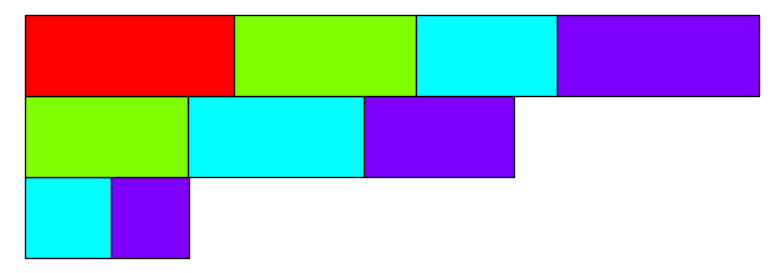
\includegraphics[height=2cm]{pplot.png}\hspace{1cm}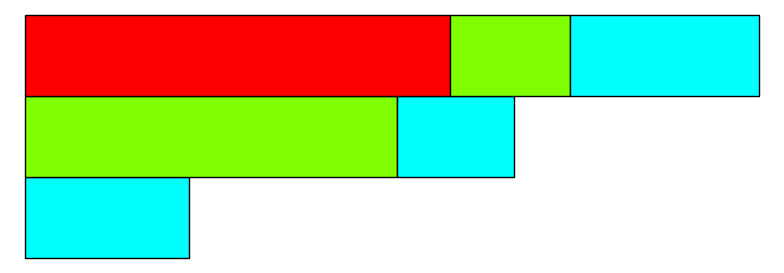
\includegraphics[height=2cm]{qplot.png}
  \end{center}
  From this visual representation, it is evident that $P$ and $Q$ are timed tableaux of the same shape.
\end{example}
\begin{theorem}
  \label{theorem:rsk}
  The function $\rsk$ defines a bijection:
  \begin{displaymath}
    \rsk: M_{m\times n}(\rp)\tilde\to \coprod_\lambda \Tab_n(\lambda)\times\Tab_m(\lambda),
  \end{displaymath}
  where $\lambda$ runs over all real partitions with at most $\min(m,n)$ parts.
\end{theorem}
\begin{remark}
  Let $\mu_i$ denote the sum of the $i$th row of $A$, and $\nu_j$ the sum of the $j$th column.
  Let $\mu=(\mu_1,\dotsc,\mu_m)$, and $\nu=(\nu_1,\dotsc,\nu_n)$.
  Then, if $\rsk(A)=(P,Q)$ then $\wt(P)=\nu$, and $\wt(Q)=\mu$.
\end{remark}
\begin{remark}[Relation to Knuth's definition]
  Knuth~\cite{knuth} defined $\rsk(A)=(P,Q)$ for integer matrices in a slightly different manner.
  His definition of $P=P(u_A)$ is exactly the same as the definition here.
  However $Q$ is defined as a \emph{recording tableau} which has the same shape as $P$ by its very construction.
  With Knuth's construction, each step (insertion followed by recording) is reversible, and it is clear that a bijection is obtained.
  The symmetry property of the RSK correspondence, that $\rsk(A^T)=(Q,P)$ if $\rsk(A)=(P,Q)$ is then stated as a non-trivial theorem.

  The definition (\ref{eq:rsk}) is the extension to real matrices of the definition in \cite[Section~18]{schur_poly} for integer matrices.
  With this definition it is immediate that if $\rsk(A)=(P,Q)$, then $\rsk(A^T)=(Q,P)$ since $u_{A^T}=v_A$.
  However, it is not immediately clear that $P$ and $Q$ have the same shape, and that the correspondence is invertible.
  These are proved using Greene's theorem in \cite{schur_poly}.
  For real matrices, the timed version of Greene's theorem allows the proof of \cite{schur_poly} to be carried out for real matrices.
  For the sake of completeness, this argument is given in full detail below.
\end{remark}
\begin{lemma}
  \label{lemma:same-shape}
  For every $A\in M_{m\times n}(\rp)$, the tableaux $P(u_A)$ and $P(v_A)$ have the same shape.
\end{lemma}
\begin{proof}
  Any timed subword $w$ of $u_A$ is of the form
  \begin{displaymath}
    w=1^{b_{11}}2^{b_{12}}\dotsb n^{b_{1n}}\,1^{b_{21}}2^{b_{22}}\dotsb n^{b_{2n}}\,\dotsb \,1^{b_{m1}}2^{b_{m2}}\dotsb n^{b_{mn}},    
  \end{displaymath}
  where $0\leq b_{ij}\leq a_{ij}$ for all $(i,j)$.
  If $w$ is a row, then the indices $(i_1,j_1),\dotsc,(i_k,j_k)$ for which $b_{ij}>0$, when taken in the order in which they appear in $w$, must satisfy $i_1\leq \dotsc \leq i_k$, and $j_1\leq \dotsb \leq j_k$.
  Define a partial order on the set
  \begin{displaymath}
    P_{mn} = \{(i,j)\mid 1\leq i\leq m,1\leq j \leq n\}
  \end{displaymath}
  by $(i,j)\leq (i',j')$ if and only if $i\leq i'$ and $j\leq j'$.
  Then it follows that the $k$th timed Greene's invariant of $u_A$ (Definition~\ref{definition:timed-Greene-invars}) is given by:
  \begin{displaymath}
    a_k(u_A) = \max_C \sum_{(i,j)\in C} a_{ij},
  \end{displaymath}
  where the maximum is taken over the set of all subsets $C\subset P_{mn}$ which can be written as a union of $k$ chains.
  Since the order relation on $P_{mn}$ corresponds to the order relation on $P_{nm}$ under $(i,j)\leftrightarrow (j,i)$, it follows that $a_k(v_A)=a_k(u_A)$ for all $k$.
  Thus, the timed version of Greene's theorem (Theorem~\ref{sec:timed-version-greene}) implies that $P$ and $Q$ have the same shape.
\end{proof}
\subsection{Insertion-Recording Algorithm for $\rsk(A)$}
\label{sec:insert-record-algor}
Given real partitions $\lambda$ and $\mu$ such that $\lambda$ interleaves $m$, and $w\in \ttab_{m-1}(\lambda)$, define the \emph{inflation of $w$ to shape $\mu$ by $m$} to be the unique tableau $\infl_\mu(w,m)$ of shape $\mu$ whose restriction to $m-1$ is equal to $w$.
In the notation of Section~\ref{sec:tabl-knuth-equiv}, $\overline{\infl_\mu(w,m)}=w$. 

Given $A\in M_n(\rp)$, let $r_{i,A} = 1^{a_{i1}}2^{a_{i2}}\dotsb n^{a_{in}}$.
Then $u_A=r_{1,A}r_{2,A}\dotsb r_{m,A}$.
\begin{center}
  \textbf{Insertion-Recording Algorithm}
\end{center}
\begin{itemize}
\item $P\ot \emptyset$, $Q\ot \emptyset$.
\item For $i=1,\dotsc, m$, repeat the following steps:
  \begin{itemize}
  \item $P\ot \ins(P, r_{i,A})$.
  \item $\lambda \ot \shape(P)$.
  \item $Q\ot \infl_\lambda(Q,i)$
  \end{itemize}
\item Return $(P, Q)$.
\end{itemize}
\begin{lemma}
  \label{lemma:insertion-rec-algo}
  For every $A\in M_{m\times n}(\rp)$, the output of the insertion-recording algorithm is $\rsk(A)$ as defined in (\ref{eq:rsk}).
\end{lemma}
\begin{proof}
  The proof is by induction on the number $m$ of rows in $A$.
  The base case of $m=1$ is trivial.

  Now suppose $A'$ denotes the submatrix consisting of the first $m-1$ rows of $A$.
  Then $u_A = u_{A'}r_{m,A}$, so that $P(u_A)=\ins(P(u_{A'}),r_{m,A})$,
  Also, the restriction $\bar v_A$ of $v_A$ to $m-1$ is $v_{A'}$.
  
  Since $v_{A'}$ is the restriction of $v_A$ to $A_{m-1}$, by Lemma~\ref{lemma:equivalence-restriction}, $P(v_{A'})$ is Knuth equivalent to the restriction of $P(v_A)$ to $A_{m-1}$.
  Theorem~\ref{theorem:unique-timed-tableaux}, implies that $P(v_{A'})$ is equal to the restriction of $P(v_A)$ to $A_{m-1}$.
  Therefore $P(v_A)=\infl_\lambda(P(v_{A'}), m)$, which is the output of the insertion-recording algorithm.
\end{proof}
\begin{proof}
  [Proof of Theorem~\ref{theorem:rsk}]
  The proof uses the fact that the insertion-recording algorithm is invertible.
  Following the notation of the proof of Lemma~\ref{lemma:insertion-rec-algo}, it suffices to recover $r_{m,A}$, $P(u_{A'})$ and $P(v_{A'})$ from $P(u_A)$ and $P(v_A)$ to reverse the insertion-recording algorithm.
  For this, observe that $P(v_{A'})$ is just the restriction of $P(v_A)$ to $A_{m-1}$.
  If $\mu$ is the shape of $P(v_{A'})$, then $(r_{m,A},P(u_{A'}))=\del_\mu(P(u_A))$ (see Definition~\ref{definition:deletion}).
\end{proof}
\subsection{Light-and-Shadows Real RSK}
\label{sec:light-and-shadows-rsk}
Viennot described a visual version of the Robinson-Schensted-Correspondence for permutations, using the \emph{light and shadows} method \cite{viennot1977forme}.
This algorithm was extended to the RSK correspondence on integer matrices by Fulton using the matrix-ball method \cite{fulton}.
Another such extension, called the VRSK algorithm, was given by the author in \cite[Chapter~3]{rtcv}.
In VRSK one can work directly with the matrices themselves, without having to draw them as configurations of points in the plane, which get unwieldy when matrices have large entries.
Another unforeseen advantage of the VRSK algorithm is that a minor variant works for real matrices, giving the correspondence of (\ref{eq:rsk}).
This new algorithm, which we call the \emph{light-and-shadows real RSK} is introduced in this section.
The piecewise linear nature of the RSK correspondence becomes clear from this algorithm.
\begin{definition}
  [Sequence of Leading Points]
  For a matrix $A\in M_{m\times n}(\rp)$, consider the set
  \begin{displaymath}
    \supp(A) = \{(i,j)\in P_{mn}\mid a_{ij}>0\}.
  \end{displaymath}
  Then the sequence $L(A)$ of leading points of $A$ is the set $\max(\supp(A))$ (with respect to the poset structure on $P_{mn}$) arranged in a sequence
  \begin{displaymath}
    L(A) = (i_1,j_1),\dotsc,(i_r,j_r)
  \end{displaymath}
  such that $j_1<\dotsb <j_r$ and (since this set is an antichain in $P_{mn}$) $i_1>\dotsb >i_r$.
\end{definition}
\begin{center}
  \textbf{Light-and-Shadows Real RSK}
\end{center}
\begin{itemize}
\item $P\ot \emptyset$, $Q\ot\emptyset$.
  \textcolor{blue}{
  \item While $A$ is non-zero repeat the following steps:
    \begin{itemize}
    \item Set $S\ot 0_{m\times n}$ ($m\times n$ zero matrix)
    \item Set $p=\emptyset$, $q=\emptyset$.
    \item While $A$ is non-zero repeat the following steps:
      \begin{itemize}
      \item Compute $L(A) = (i_1,j_1),\dotsc,(i_r,j_r)$ of $A$
      \item Let $m(A)=\min\{a_{i_1j_1},\dotsc,a_{i_r,j_r}\}$
      \item Set $a_{i_s,j_s}\ot a_{i_s,j_s}-m(A)$ for $s=1,\dotsc r$
      \item Set $s_{i_{s+1},j_s}\to s_{i_{s+1},j_s}+m$ for $s=1,\dotsc,r-1$
      \item Set $p\ot pj_1^m$, $q\ot q_{i_r}^m$
      \end{itemize}
    \item $P\ot pP$, $Q\ot qQ$
    \item $A\ot S$
    \end{itemize}
  }
\item Return $(P, Q)$
\end{itemize}
\begin{theorem}
  When the light-and-shadows real RSK algorithm is applied to $A\in M_{m\times n}(\rp)$, it return $\rsk(A)$.
\end{theorem}
\begin{proof}
  For the proof, we introduce an algorithm that is midway between the insertion-recording algorithm of Section~\ref{sec:insert-record-algor} and the light-and-shadows real RSK.
  \begin{center}
    \textbf{Row-wise RSK Algorithm}
  \end{center}
  \begin{itemize}
  \item $P\ot \emptyset$, $Q\ot \emptyset$
    \textcolor{blue}{
    \item While $A$ is non-zero repeat the following steps:
      \begin{itemize}
      \item Set $p\ot \emptyset$, $q\ot \emptyset$
      \item For $i=1,\dotsc,m$, repeat the following steps:
        \begin{itemize}
        \item Set $S\ot 0_{m\times n}$.
        \item Set $(v,u)=\rowins(p,1^{a_{i1}}\dotsb n^{a_{in}})$
        \item If $v=1^{s_1}\dotsb n^{s_n}$, set $s_{ij}\ot s_j$ for $j=1,\dotsc,n$.
        \end{itemize}
      \item Set $A\ot S$.
      \item $P\ot pP$, $Q\ot qQ$.
      \end{itemize}
      }
    \item return $(P, Q)$
  \end{itemize}
  The main loop of this algorithm starts with a matrix $A$, and replaces with the matrix $S=s_{ij}$ computed using timed row insertion.
  It also computes the first row of the tableau $P$ and $Q$ as $p, q$.
  We claim that the function $A\mapsto (S, p, q)$ of the main loop of the row-wise RSK algorithm is the same as the function $A\mapsto (S, p, q)$ of the main loop of the light-and-shadows real RSK.
  We call $S$ the \emph{shadow matrix} of $A$.

  Write $A$ as a block matrix $\binom{A'}{A''}$, where $A'$ is an $(m-1)\times n$ matrix and $A''$ is a $1\times n$ matrix.
  It suffices to show that if the light-and-shadows real RSK algorithm return $(P',Q')$ on $A'$ and $(P, Q)$ on $A$, the $P=\ins(P',u_{A''})$.
  Here $u_{A''}$ is just the row:
  \begin{displaymath}
    1^{a_{m1}}\dotsb n^{a_{mn}}.
  \end{displaymath}

  The inner loop of the light-and-shadows real RSK algorithm produces a sequence $A'=A'_1, A'_2,\dotsc, A'_h$ of matrices as it runs on input $A'$.
  Let $L'_k=L(A'_k)$ and $m'_k=m(A'_k)$, for $k=1,\dotsc,h$.
  When the inner loop finishes running, we have $p'={j'_1}^{m'_1}\dotsb {j'_h}^{m'_h}$, and $q' = {i'_1}^{m'_1}\dotsb {i'_h}^{m'_h}$, where $j'_k$ is the least non-zero column, and $i'_k$ is the least non-zero row of $A'_k$.


  Now $A$ is obtained from $A'$ by adding a new row
  $
  \begin{pmatrix}
    a_{m1}&\dotsb & a_{mn}
  \end{pmatrix}
  $.
  To begin with, assume that this row has only one non-zero entry, $a_{mj_0}$.
  Let $L_1,L_2,\dotsc$, and $m_1,m_2,\dotsc$ be the corresponding sequences of leading 
  If $j_0\geq j_i$ for all $i$, then $L_k=L'_k$ for all $k=1,\dotsc,h$.
  In addition, $A$ has a singleton sequence of leading points $\{(m,j_0)\}$.
  As a result, the output of the main loop is $p=p'u_{A''}$, and $q=q'm^{a_{mj_0}}$, and the shadow matrix of $A$ is the same as the shadow matrix of $A'$.
  The same outcome is obtained from the main loop of the row-wise RSK algorithm.
  The hypothesis that $j_0\geq j_i$ for all $i$ is equivalent to saying that $A''$ has its non-zero entries to the left of any non-zero entries of $A'$.
  Therefore $P(u_A)=P(u_{A'})u_{A''}$, and the shadow matrix of $A'$ generated by row-wise RSK is the same as the shadow matrix of $A$ generated by row-wise RSK.
  
  Now suppose that $j_0<j_l$ for some $l$, and take the least such value $l$.
  Then the sequences of leading points $L_1,\dotsc,L_{l-1}$ of $A$ are the same as the sequences $L'_1,\dotsc,L'_{l-1}$.
  If $a_{mj_0}\geq m'_{j'_l}+\dots m'_{j'_h}$, then $L_k=\{(m,j_0)\}\cup L'_k$ for $k=l,\dotsc, h$.
  Therefore $p={j'_1}^{m'_1}\dotsb {j'_{l-1}}^{m'_{l-1}}j_0^{a_{mj_0}}$.
  From the definition of timed row insertion (Definition~\ref{definition:timed-row-insertion}), $\rowins(p',j_0^{a_{mj_0}}) = (j_l^{m_l}\dotsb j_h^{m_h},p)$.
  Also, $q=q'm^{a_{mj_0}}$.
  Finally, $S$ is obtained from $S'$ by adding $m'_k$ to the $(m,j_k)$th entry of $S'$ for each $k=l,\dotsc,h$.

  Otherwise, $m_{j_l}+\dotsb+m_{j_{q-1}}<a_{mj_0}\leq m_{j_1}+\dotsb+m_{j_q}$ for some $l\leq q<h$.
  In this case the sequences of leading points for $A$ are given by:
  \begin{displaymath}
    L_k =
    \begin{cases}
      L'_k & \text{for } 1\leq k<l-1,\\
      (m,j_0)\cup L'_k & \text{for } l\leq k\leq q,\\
      L'_{k-1} & \text{for } q\leq l\leq h,
    \end{cases}
  \end{displaymath}
  $p={j'_1}^{m'_1}\dotsb j_{l-1}^{m'_{l-1}}j_0^{a_{m0}}j_q^{m'_{j_1}+\dotsb + m'_{j_q}-a_{mj_0}}j_{q+1}^{m'_{q+1}}\dotsb j_h^{m'_h}$.
  Again from the definition of timed row insertion, $\rowins(p',j_0^{a_{mj_0}}) = (j_l^{m'_l}\dotsb j_{q-1}^{m'_{q-1}}j_q^{a_{mj_0}-(m'_1+\dotsb+m'_{l-1})}, p)$.
  Also, $q=q'm^{a_{mj_0}}$.
  Finally, the value $m'_k$ is added to the $(m,j_k)$th entry of $S'$ for $k=l,\dotsc,q-1$, and $a_{mj_0}-(m'_1+\dotsb+m'_{l-1})$ is added to the $(m,j_q)$th entry of $S'$ to obtain $S$.

  Thus we have seen that when $A''$ has a single non-zero entry, the effect of this entry modifies the outputs of both the row-wise real RSK algorithm and the light-and-shadows real RSK algorithm in exactly the same manner.

  If the last row of $A$ has more than one non-zero entry, they may be dealt with sequentially (from left to right) to get the same outcome.
\end{proof}
\subsection{Piecewise Linear RSK}
\label{sec:piecewise-linear-rsk}
\begin{definition}
  [Gelfand-Tsetlin Pattern]
  A Gelfand-Tsetlin pattern of size $n$ is a triangle $T=(\lambda^{(k)}_i\mid 1\leq k \leq n, 1\leq i \leq k)$ of nonegative real numbers:
  \begin{displaymath}
    \begin{matrix}
      \lambda^{(n)}_1 & & \lambda^{(n)}_2 && \dotsb && \dotsb && \lambda^{(n)}_n\\
      &\lambda^{(n-1)}_1 && \lambda^{(n-1)}_2 && \dotsb && \lambda^{(n-1)}_{n-1} & \\
      && \ddots && \ddots && \udots &&  \\
      &&& \ddots && \udots &&&\\
      &&&& \lambda^{(1)}_1 &&&&
    \end{matrix}
  \end{displaymath}
  such that $\lambda^{(k)}_i\geq \lambda^{(k-1)}_i\geq \lambda^{(k)}_{i+1}$ for $k=2,\dotsc,n$ and $i=1,\dotsc, k-1$.
  The shape of a Gelfand-Tsetlin pattern of size $n$ is its \emph{top row}, $\lambda^{(n)}$.
\end{definition}
Whenever $n\geq k$, define $r^n_k:A_n^\dagger\to A_k^\dagger$ by taking $r^n_k(w)$ to be the timed word whose exponential string is obtained from the exponential string of $w$ by deleting all terms of the form $c^t$ where $c>k$.
It is easy to see that if $w\in A_n^\dagger$ is a timed tableau, then so is $r^n_k(w)$ for all $k=1,\dotsc,n$.

In this section, given a timed tableau $w$ in $A_n$, its shape will always be written as a real partition with $n$ components, $\lambda=(\lambda_1,\dotsc,\lambda_n)$, where $\lambda_1\geq \dotsb \lambda_n\geq 0$.

Given a timed tableau $w$ in $A_n$, define partitions $\lambda^{(k)}=(\lambda^{(k)}_1,\dotsc,\lambda^{(k)}_k)$ by $\lambda^{(k)} = \shape(r^n_k(w))$.
By Lemma~\ref{lemma:restriction-interleaf}, $\lambda_{(k-1)}$ interleaves $\lambda^{(k)}$ for all $k=2,\dotsc,n$.
Therefore the numbers $\lambda^{(k)}_i$ form a Gelfand-Tsetlin pattern, which we denote by $GT(w)$.
The shape of $\lambda$ is also the shape of $GT(w)$.
Conversely, given a Gelfand-Tsetlin pattern $T$, it is easy to reconstruct the unique timed tableau $w$ such that $T=GT(w)$.

The space of all Gelfand-Tsetlin patterns of size $n$, being defined by a finite collection of homogeneous inequalities in $\binom{n+1}2$ variables, forms a polydedral cone in $R^{\binom{n+1}2}$.
In terms of the notation introduced in Section~\ref{sec:defin-using-timed}, we have the following fairly lemma, which is well-know for the RSK correspodnece on integer matrices (see e.g., \cite[Prop.~2.26]{kir-trop}).
\begin{lemma}
  \label{lemma:pl}
  Given $A\in M_{m\times n}(\rp)$ with $\rsk(A)=(P,Q)$, let $(\lambda^{(k)}_i)=GT(P)$ and $(\mu^{(k)}_i)=GT(Q)$, Gelfand-Tsetlin patterns of size $n$ and $m$ respectively.
  Then
  \begin{align}
    \label{eq:gt-1}
    \lambda^{(j)}_1 + \dotsb \lambda_k^{(j)} & = \max_{C\subset P_{mj}\text{ union of at most $k$ chains}} \sum_{(i,j)\in C} a_{ij},\\
    \label{eq:gt-2}
    \mu_1^{(i)} + \dotsb + \mu_k^{(i)} & = \max_{C\subset P_{in}\text{ union of at most $k$ chains}} \sum_{(i,j)\in C} a_{ij},
  \end{align}
  for all $1\leq j\leq n$, and $1\leq i\leq m$.
\end{lemma}
\begin{proof}
  Let $A_j$ is the submatrix of $A$ consisting of its first $j$ columns, then $u_{A_j} = r^n_j(u_A)$.
  By a repeated application of Lemma~\ref{lemma:equivalence-restriction}, $P(u_{A_j}) = r^n_j(P(u_A))$.
  But the $j$ row of $GT(P)$ is, by definition, the shape of $r^n_j(P(u_A))$.
  But the shape of $P(u_{A_j})$ is given by (\ref{eq:gt-1}), as explained in the proof of Lemma~\ref{lemma:same-shape}.
  The identity (\ref{eq:gt-2}) has a similar proof.
\end{proof}
\begin{corollary}
  The RSK correspondence defines a continuous piecewise linear bijection from the cone $M_{m\times n}(\rp)$ onto the cone of pairs of Gelfand-Tsetlin patterns $((\lambda^{(k)}_i), (\mu^{(k)}_i))$ of sizes $n$ and $m$ respectively, with $\lambda^{(n)}=\mu^{(m)}$ (after padding the shorter of the two with zeros).
\end{corollary}
Lemma~\ref{lemma:pl} clearly demonstrates the piecewise linear nature of the RSK correspondence:
The algorithms of Sections~\ref{sec:defin-using-timed}--\ref{sec:light-and-shadows-rsk} allow for fast computations of this piecewise linear map.
While Eqs.~(\ref{eq:gt-1}) and (\ref{eq:gt-2}) are used to \emph{define} the RSK correspondence in \cite{kir-trop}, in this article, the RSK \emph{algorithm} is extended to real matrices, and Lemma~\ref{lemma:pl} is proved for the extended algorithm.

A more detailed analysis of the piecewise linear nature of the real RSK correspondence will be carried out in \cite{cgp}.
\subsection{Note on software}
\label{sec:software}
All the algorithms in this article are demonstrated using python code.
This includes an implementation of classes of timed words, timed rows, and timed tableau (with methods for concatenation, insertion, construction of insertion tableau, and many other operations).
It also includes an implementation of the RSK correspondence and its inverse.
The code is available at \url{http://www.imsc.res.in/~amri/timed_plactic/timed_tableau.py}.

The code is accompanying by a demo jupyter worksheet, where the use of all these algorithms is illustrated.
The worksheet also includes verifications of all the theorems in this paper using randomized inputs.
The worksheet is available at \url{http://www.imsc.res.in/~amri/timed_plactic/timed_tableau.ipynb}.
\bibliographystyle{abbrv}
\bibliography{refs}
\end{document}
